\documentclass{article}

\title{Chapter 25: Capacitance}
\author{Rylan Polster}

\usepackage[parfill]{parskip}
\usepackage{multirow}
\usepackage{amsmath,amssymb,amsthm}
\usepackage{bm}
\usepackage{textcomp,gensymb}
\usepackage{siunitx}
\usepackage{graphicx,float,caption}
\graphicspath{ {images/} }
\captionsetup{width=\linewidth}
\usepackage[margin=1.0in]{geometry}

\begin{document}
    \maketitle
    
    \section*{General}

        \paragraph{Quantities}
        \begin{align}
            q &= \text{charge} \nonumber\\
            V &= \text{electric potential} \nonumber\\
            C &= \text{capacitance} \nonumber\\
            U &= \text{electric potential energy} \nonumber\\
            W &= \text{work} \nonumber\\
            \vec{E} &= \text{electric field} \nonumber\\
            d &= \text{plate separation} \nonumber\\
            A &= \text{plate area} \nonumber\\
            L &= \text{length of a cylindrical capacitor} \nonumber\\
            a &= \text{inner radius of a cylindrical or spherical capacitor} \nonumber\\
            b &= \text{outer radius of a cylindrical or spherical capacitor} \nonumber\\
            \epsilon_0 &= \text{vacuum permittivity constant} \nonumber\\
            \kappa &= \text{dielectric constant} \nonumber
        \end{align}

        \paragraph{Constants}
        \begin{align}
            \epsilon_0 &= \SI[per-mode=fraction]{8.85e-12}{\farad\per\meter} \nonumber
        \end{align}

    \section{Capacitance}

        A capacitor is a device in which electrical energy can be stored. A capacitor is comprised of two isolated conductors of any shape. The plates (the term plate is used regardless of the shape of the capacitor) can be charged to the same magnitude of charge with opposite signs ($+q$ and $-q$).

        \paragraph{Capacitance} Capacitance ($C$) is a measure of how much charge can be put on the plates to produce a certain potential difference between them. The greater the capacitance, the more charge is required. The capacitance is measured in farads ($\si{\farad}$).
        \begin{equation}
            \SI{1}{\farad} = \SI[per-mode=fraction]{1}{\coulomb\per\volt}
        \end{equation}
        \begin{equation}
            q = C V
        \end{equation}

    \section{Calculating the Capacitance}

        \paragraph{Electric Field}
        \begin{equation}
            E = \frac{1}{4\pi\epsilon_0} \frac{q}{d^2}, \quad V = \frac{1}{4\pi\epsilon_0} \frac{q}{d} \nonumber
        \end{equation}
        \begin{equation}
            E = \frac{V}{d}
        \end{equation}
        \begin{equation}
            q = \epsilon_0 E A
        \end{equation}

        \paragraph{Parallel Plate Capacitor}
        \begin{equation}
            C = \frac{\epsilon_0 A}{d}
        \end{equation}

        \paragraph{Cylindrical Capacitor}
        \begin{equation}
            C = 2 \pi \epsilon_0 \frac{L}{\ln(b/a)}
        \end{equation}

        \paragraph{Spherical Capacitor}
        \begin{equation}
            C = 4 \pi \epsilon_0 \frac{ab}{b-a}
        \end{equation}

    \section{Capacitors in Parallel and in Series}

        \paragraph{Capacitors in Parallel}
        When a potential difference $V$ is applied across several capacitors connected in parallel, that potential difference $V$ is applied across each capacitor. The total charge $q$ stored on the capacitors is the sum of the charges stored on all the capacitors.

        \begin{figure}[H]
            \centering
            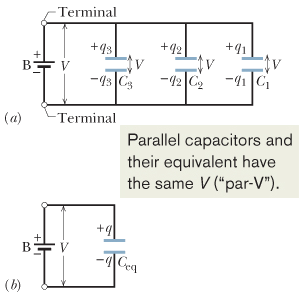
\includegraphics[scale=0.6]{parallel}
            \caption{Three capacitors connected in parallel to battery B. The battery maintains potential difference $V$ across its terminals and thus across each capacitor. The equivalent capacitor, with capacitance $C_{eq}$, replaces the parallel combination. (see equation \ref{eq:parallel})}
        \end{figure}

        Capacitors connected in parallel can be replaced with an equivalent capacitor that has the same total charge $q$ and the same potential difference $V$ as the actual capacitors.

        \begin{equation} \label{eq:parallel}
            C_{eq} = \sum_{j=1}^n C_j
        \end{equation}
        \begin{equation}
            q_{eq} = \sum_{j=1}^n q_j
        \end{equation}
        \begin{equation}
            U_{eq} = \sum_{j=1}^n U_j
        \end{equation}

        \paragraph{Capacitors in Series}
        When a potential difference $V$ is applied across several capacitors connected in series, the capacitors have identical charge $q$. The sum of the potential differences across all the capacitors is equal to the applied potential difference $V$.

        \begin{figure}[H]
            \centering
            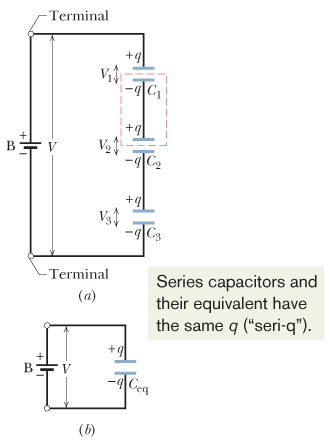
\includegraphics[scale=0.6]{series}
            \caption{Three capacitors connected in series to battery B. The battery maintains potential difference $V$ between the top and bottom plates of the series combination. The equivalent capacitor, with capacitance $C_{eq}$, replaces the parallel combination. (see equation \ref{eq:series})}
        \end{figure}

        Capacitors that are connected in series can be replaced with an equivalent capacitor that has the same charge $q$ and the same total potential difference $V$ as the actual series capacitors.

        \begin{equation} \label{eq:series}
            \frac{1}{C_{eq}} = \sum_{j=1}^n \frac{1}{C_j}
        \end{equation}
        \begin{equation}
            V_{eq} = \sum_{j=1}^n V_j
        \end{equation}
        \begin{equation}
            U_{eq} = \sum_{j=1}^n U_j
        \end{equation}

    \section{Energy Stored in an Electric Field}

        \paragraph{Work}
        The work required to bring the total capacitor charge up to a final value $q$ is:
        \begin{equation}
            dW = V' \, dq' = \frac{q'}{C} \, dq' \nonumber
        \end{equation}
        \begin{equation}
            W = \int dW = \frac{1}{C} \int_0^q q' \, dq' = \frac{q^2}{2C} \nonumber
        \end{equation}

        \paragraph{Potential Energy}
        The work is stored as potential energy in the capacitor.
        \begin{equation}
            U = \frac{q^2}{2C} = \frac{1}{2}CV^2 = \frac{1}{2}qV
        \end{equation}

        \paragraph{Energy Density}
        The energy density is the potential energy per unit volume between the plates.
        \begin{equation}
            u = \frac{U}{\text{volume}} = \frac{U}{Ad} = \frac{CV^2}{2Ad} \nonumber
        \end{equation}
        \begin{equation}
            u = \frac{1}{2} \epsilon_0 \left(\frac{V}{d}\right)^2 \nonumber
        \end{equation}
        \begin{equation}
            u = \frac{1}{2} \epsilon_0 E^2
        \end{equation}

    \section{Capacitors with a Dielectric}

        \begin{equation}
            C = \kappa C_\text{air}
        \end{equation}

        In a region completely filled by a dielectric material of dielectric constant $\kappa$, all electrostatic equations containing the permittivity constant $\epsilon_0$ are to be modified by replacing $\epsilon_0$ with $\kappa$.

\end{document}
